\documentclass{beamer}

\usepackage{graphicx} % Allows including images
\usepackage{booktabs} % Allows the use of \toprule, \midrule and \bottomrule in tables

% Use the preamble from the main paper if desired
% % Conveniently, the citeautoscript option in the revtex4-2 class toggles the spacing & punctuation automatically for superscript vs. bracketed citations. Place citations as if they were in [].
% Uncomment the line below to do superscript citations.
% \setcitestyle{super}

\usepackage{amsmath,amssymb} % math symbols
\usepackage{bm} % bold math font
\usepackage{graphicx} % for figures
\usepackage{comment} % allows block comments
\usepackage[normalem]{ulem} % allows strikeout text, e.g. \sout{text}

% \usepackage{minted} % allows colored code
% \usepackage{textcomp} % This package gives the text quote '

\usepackage{enumitem}
\setlist{noitemsep,leftmargin=*,topsep=0pt,parsep=0pt}

\usepackage{xcolor} % \textcolor{red}{text} will be red for notes
\definecolor{lightgray}{gray}{0.6}
\definecolor{medgray}{gray}{0.4}
\definecolor{mRed}{RGB}{230, 0, 50}
\colorlet{newtextColor}{mRed}

\usepackage{hyperref}
\hypersetup{
colorlinks=true,
urlcolor= blue,
citecolor=blue,
linkcolor= blue,
}

% Code to add paragraph numbers and titles
\newif\ifptitle
\newif\ifpnumber
\newcounter{para}
\newcommand\ptitle[1]{\par\refstepcounter{para}
{\ifpnumber{\noindent\textcolor{lightgray}{\textbf{\thepara}}\indent}\fi}
{\ifptitle{\textbf{[{#1}]}}\fi}}
%\ptitletrue  % comment this line to hide paragraph titles
%\pnumbertrue  % comment this line to hide paragraph numbers

% Code for reviewer text
%\newcommand{\revtext}[1]{\textcolor{reviewColor}{#1}}
\newcommand{\revtext}[1]{\textit{#1}}

% Code to track changes
\newif\iftrackchanges
\newcommand{\newtext}[1]
    {\textcolor{\iftrackchanges newtextColor\else black\fi}{#1}}
\newcommand{\deltext}[1]
    {\iftrackchanges{\textcolor{newtextColor}{\sout{#1}}}\fi}
%\trackchangestrue  % comment to hide tracked changes

% Instead of making TONS of colored newtext, let's just put a colored line next to big blocks of new text.
\usepackage{mdframed}
\newmdenv[
  linecolor={\iftrackchanges newtextColor\else white\fi},
  linewidth=2pt,
  topline=false,
  bottomline=false,
  rightline=false,
  skipabove=\topsep,
  skipbelow=\topsep,
  leftmargin=-12pt,
  innertopmargin=0pt,
  innerbottommargin=0pt
]{newtextblock}

% Uncomment this line if you prefer your vectors to appear as bold letters.
% By default they will appear with arrows over them.
% \renewcommand{\vec}[1]{\bm{#1}}

% Command to mark text in blue/red and define common units
\newcommand{\blue}[1]{\textcolor{blue}{#1}}
\newcommand{\red}[1]{\textcolor{red}{#1}}
\newcommand{\df}{\dfrac}
\newcommand{\mic}{\mu\mathrm{m}}
\newcommand{\nm}{\mathrm{nm}}
\newcommand{\mm}{\mathrm{mm}}
\newcommand{\mrm}[1]{\mathrm{#1}}
\newcommand{\la}{\langle}
\newcommand{\ra}{\rangle}
\newcommand{\pd}[1]{\partial_{#1}}
% Command for labeled equations with custom alignment
\newcommand{\leqalign}[2]{
    \begin{equation}
        \begin{aligned}
            #2
        \end{aligned}
        \label{#1}
    \end{equation}
}
 
% % Conveniently, the citeautoscript option in the revtex4-2 class toggles the spacing & punctuation automatically for superscript vs. bracketed citations. Place citations as if they were in [].
% Uncomment the line below to do superscript citations.
% \setcitestyle{super}

\usepackage{amsmath,amssymb} % math symbols
\usepackage{bm} % bold math font
\usepackage{graphicx} % for figures
\usepackage{comment} % allows block comments
\usepackage[normalem]{ulem} % allows strikeout text, e.g. \sout{text}

% \usepackage{minted} % allows colored code
% \usepackage{textcomp} % This package gives the text quote '

\usepackage{enumitem}
\setlist{noitemsep,leftmargin=*,topsep=0pt,parsep=0pt}

\usepackage{xcolor} % \textcolor{red}{text} will be red for notes
\definecolor{lightgray}{gray}{0.6}
\definecolor{medgray}{gray}{0.4}
\definecolor{mRed}{RGB}{230, 0, 50}
\colorlet{newtextColor}{mRed}

\usepackage{hyperref}
\hypersetup{
colorlinks=true,
urlcolor= blue,
citecolor=blue,
linkcolor= blue,
}

% Code to add paragraph numbers and titles
\newif\ifptitle
\newif\ifpnumber
\newcounter{para}
\newcommand\ptitle[1]{\par\refstepcounter{para}
{\ifpnumber{\noindent\textcolor{lightgray}{\textbf{\thepara}}\indent}\fi}
{\ifptitle{\textbf{[{#1}]}}\fi}}
%\ptitletrue  % comment this line to hide paragraph titles
%\pnumbertrue  % comment this line to hide paragraph numbers

% Code for reviewer text
%\newcommand{\revtext}[1]{\textcolor{reviewColor}{#1}}
\newcommand{\revtext}[1]{\textit{#1}}

% Code to track changes
\newif\iftrackchanges
\newcommand{\newtext}[1]
    {\textcolor{\iftrackchanges newtextColor\else black\fi}{#1}}
\newcommand{\deltext}[1]
    {\iftrackchanges{\textcolor{newtextColor}{\sout{#1}}}\fi}
%\trackchangestrue  % comment to hide tracked changes

% Instead of making TONS of colored newtext, let's just put a colored line next to big blocks of new text.
\usepackage{mdframed}
\newmdenv[
  linecolor={\iftrackchanges newtextColor\else white\fi},
  linewidth=2pt,
  topline=false,
  bottomline=false,
  rightline=false,
  skipabove=\topsep,
  skipbelow=\topsep,
  leftmargin=-12pt,
  innertopmargin=0pt,
  innerbottommargin=0pt
]{newtextblock}

% Uncomment this line if you prefer your vectors to appear as bold letters.
% By default they will appear with arrows over them.
% \renewcommand{\vec}[1]{\bm{#1}}

% Command to mark text in blue/red and define common units
\newcommand{\blue}{\textcolor{blue}}
\newcommand{\red}[1]{\textcolor{red}{#1}}
\newcommand{\df}{\dfrac}
\newcommand{\mic}{\mu\mathrm{m}}
\newcommand{\nm}{\mathrm{nm}}
\newcommand{\mm}{\mathrm{mm}}
\newcommand{\mrm}[1]{\mathrm{#1}}
\newcommand{\la}{\langle}
\newcommand{\ra}{\rangle}
\newcommand{\pd}[1]{\partial_{#1}}
% Command for labeled equations with custom alignment
\newcommand{\leqalign}[2]{
    \begin{equation}
        \begin{aligned}
            #2
        \end{aligned}
        \label{#1}
    \end{equation}
}


\title[NV Center Presentation]{Optical Characterization and Coherent Control of Single NV Centers} % The short title appears at the bottom of every slide, the full title is only on the title page
\author{Adam Pearl \and Nicholas Lyu}
\institute[Harvard Physics]{Department of Physics \\ Harvard University}
\date{\today} % Date, can be changed to a custom date
\usepackage{siunitx}
\begin{document}

\begin{frame}
\titlepage % Print the title page as the first slide
\end{frame}

% \begin{frame}
% \frametitle{Overview}
% \tableofcontents % This will list sections and subsections
% \end{frame}

%------------------------------------------------
\section{Introduction}

\begin{frame}
    \frametitle{Introduction: NV Centers}
    \begin{itemize}
        \item Substitutional Nitrogen + Vacancy $\rightarrow$ NV$^{-}$ state \cite{doherty2013nitrogen}
        \item Significance: Quantum sensing and information processing
    \end{itemize}
    \begin{figure}
        \centering
        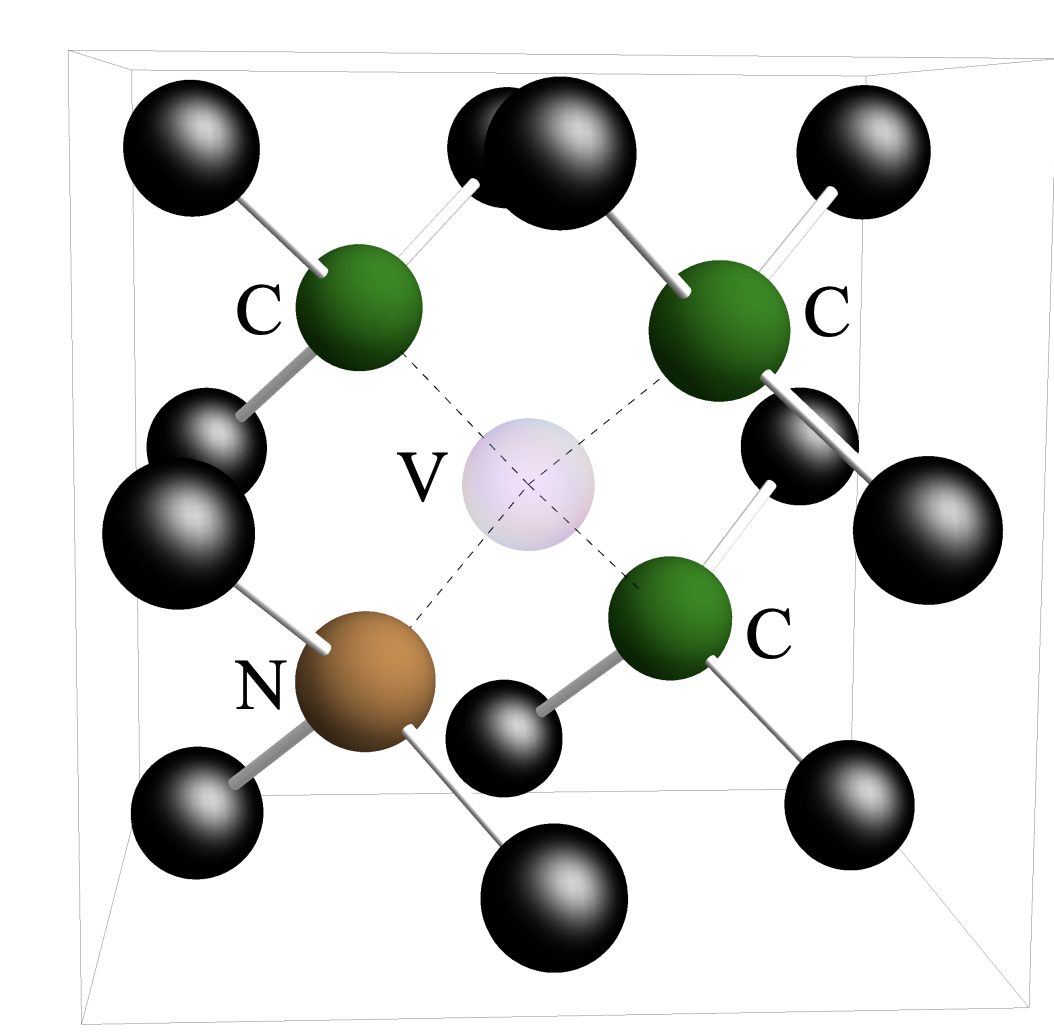
\includegraphics[width=0.5\textwidth]{./figs/lattice.png} % Adjust width as needed
        \caption{Schematic of the NV center structure in the diamond lattice \cite{doherty2013nitrogen}.}
        \label{fig:nv_structure_pres}
    \end{figure}
\end{frame}

\begin{frame}
    \frametitle{NVs Continued} 
    \begin{itemize}
        \item Ground state manifold: effective spin-1 triplet $|m_s=0, \pm 1\rangle$
        \item Effective spin Hamiltonian $H = D\, S_z^2 + \gamma_e {\mathbf{B}} \cdot {\mathbf{S}}$ \cite{Prasad2018NVNotes}. 
        \begin{itemize}
            \item $D$: zero-field splitting between $|0\rangle$ and $|\pm 1\rangle$. 
            \item Typical value $2.87$ GHz at $\SI{300}{\kelvin}$. 
        \end{itemize}
    \end{itemize}
    \begin{table}
        \centering
        {\small % Decrease entire table font size by 1pt (to 10pt)
        \begin{tabular}{ll>{\scriptsize}l} % Decrease last column font size to scriptsize (8pt)
            \toprule
            Source & Specs & Effect \\
            \midrule
            NdYAG laser & \SI{532}{\nano\meter} & 
            Pumps ground to excited manifold. \\ 
             & & Relaxes to $|0\rangle$ by fluorescence and phonon emission. \\
            Microwave & $\sim$\SI{2.87}{\giga\hertz} & Drives transitions between $|0\rangle$ and $|\pm 1\rangle$. \\
            \bottomrule
        \end{tabular}
        } % End \small scope
        % \caption{Radiation sources and their effects on NV center states.}
        \label{tab:radiation_effects}
    \end{table}
\end{frame}

\begin{frame}
    \frametitle{NVs (Finally)} 
    Net effect of exciting a NV center with a green laser: 
    \begin{itemize}
        \item $|m_s=0\rangle$: fluoresces with high probability, returns in $|0\rangle$. 
        \begin{itemize}
            \item Red fluorescence due to phonon + photon emission (PSB). 
        \end{itemize}
        \item $|m_s=\pm 1\rangle$: Relax to $|0\rangle$ by emitting phonons. 
        \begin{itemize}
            \item Little fluorescence due to phonon emission (ISC). 
        \end{itemize}
    \end{itemize}
    
\end{frame}

%------------------------------------------------
\section{Setup}

\begin{frame}
\frametitle{Experimental Setup Overview}
\begin{itemize}
    \item Confocal Microscope: Laser (532nm), Objective (NA 1.3), Dichroic, Filters, APDs.
    \item Scanning: Galvanometers (XY), Piezo (Z).
    \item Microwave Delivery: source, amplifier, antenna. 
    \item Control: LabVIEW, DAQ card, pulse generator. 
\end{itemize}
\begin{figure}
    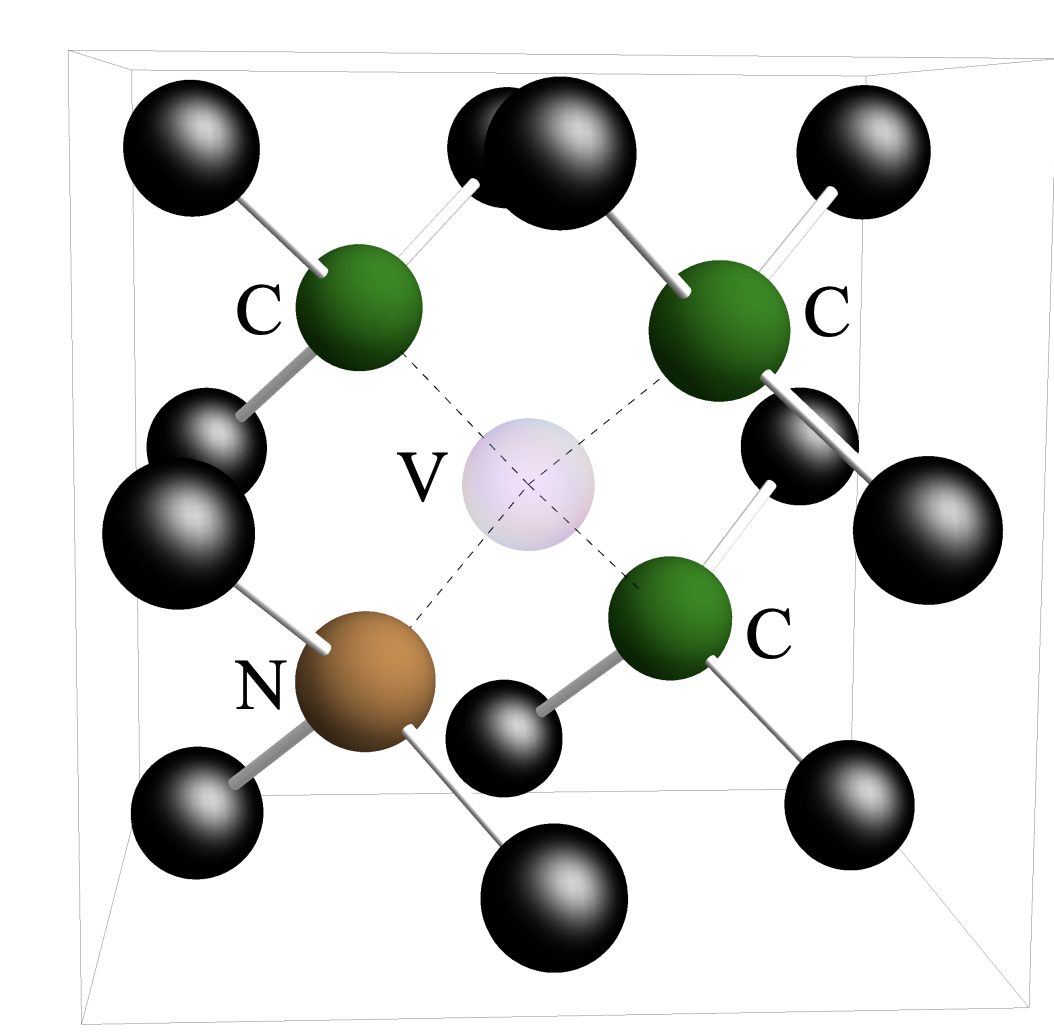
\includegraphics[width=0.7\textwidth]{figs/lattice.png} % Adjust path if needed
    \caption{Experiment setup (Placeholder)}
    \end{figure}
\end{frame}

%------------------------------------------------
% \section{$g^{(2)}$ Measurement}

\begin{frame}
\frametitle{$g^{(2)}$ Measurement: Theory}
\begin{itemize}
    \item Purpose: Confirm single photon emission.
    \item Hanbury Brown and Twiss (HBT) Setup: 50/50 beamsplitter, two detectors (APDs).
    \item Measure time correlations between photon arrivals.
    \item Second-order correlation function $g^{(2)}(\tau) = \frac{\langle I(t)I(t+\tau) \rangle}{\langle I(t) \rangle^2}$
    \item Expectation for single emitter: $g^{(2)}(0) < 1$ (ideally 0). Antibunching.
    \item Expectation for classical light: $g^{(2)}(0) \ge 1$.
\end{itemize}
\end{frame}

\begin{frame}
\frametitle{$g^{(2)}$ Measurement: Result}
\begin{itemize}
    \item Experimental histogram of photon arrival time differences.
    \item Clear dip observed near $\tau = 0$: single photon emitter!
\end{itemize}
% Add g(2) histogram figure
% \begin{figure}
% \includegraphics[width=0.7\textwidth]{../first_draft/figs/g2_histogram.png} % Adjust path if needed
% \caption{$g^{(2)}(\tau)$ measurement showing antibunching.}
% \end{figure}
\end{frame}
% \section{Coherent Control}

\begin{frame}
    \frametitle{Rabi preliminary: driving two-level systems}
    \begin{itemize}
        \item Simplified Hamiltonian: $H \propto \dfrac{\omega_0}{2} \sigma_z + \dfrac{\omega_1}{2} \cos(\omega t + \phi) \sigma_x$
        \begin{itemize}
            \item $\omega_0$: two-level energy splitting (e.g. $|0\rangle$ and $|1\rangle$ in NV). 
            \item $\omega_1$: energy of the microwave drive. 
            \item $\omega$: driving frequency. 
        \end{itemize}

        \item Switch to a rotating frame with $U(t) = e^{-i\omega t \sigma_z/2}$. 
        \begin{align*}
            H(t) 
            &\mapsto i \dot U(t)U(t)^\dag + U(t) H(t) U(t)^\dag = \dots \\ 
            &= \dfrac 1 2 \Omega \, \vec n\cdot \vec \sigma + (\text{time-dependent ignorable terms})
        \end{align*}
        \item $\Omega = \sqrt{\omega_1^2/4 + (\omega - \omega_0)^2}$: Rabi frequency. 
        \item $\vec{n} = \left[\frac{\omega_1 \cos \varphi}{2\Omega}, -\frac{\omega_1 \sin \varphi}{2\Omega}, \frac{\omega_0-\omega}{2\Omega}\right]$: rotation axis. 
    \end{itemize}
\end{frame}

\begin{frame}
\frametitle{Rabi Oscillations}
\begin{itemize}
    \item Rabi takeaways: \underline{in the rotating frame}, 
    \begin{itemize}
        \item \textcolor{blue}{Free evolution $=$ rotation by $z$-axis.} 
        \item \textcolor{blue}{Microwave drives rotation about $\vec{n}$ with angular frequency $\Omega$.} 
    \end{itemize}
    \item Pulse Sequence: Init (Laser) - MW($t$) - Readout (Laser)
    \begin{itemize}
        \item Assuming zero detuning, coherently drives spin between $|0\rangle$ and $|1\rangle$. 
        \item Observe oscillations in fluorescence (PL) vs $t$.
    \end{itemize}
    \item PL$(t) \propto \cos(\Omega_R t + \phi) \exp(-t/T_{Rabi})$. $\Omega_R$: Rabi frequency.
\end{itemize}
% Add Rabi figure
% \begin{figure}
% \includegraphics[width=0.7\textwidth]{../first_draft/figs/rabi.png} % Adjust path if needed
% \caption{Rabi oscillations.}
% \end{figure}
\end{frame}

\begin{frame}
\frametitle{Hahn Echo}
\begin{itemize}
    \item Pulse Sequence: Init - $\pi/2$ - Free Evolution($\tau$) - $\pi$ - Free Evolution($\tau$) - $\pi/2$ - Readout
    \begin{itemize}
        \item $\pi$-pulse adjusts for the effects of quasi-static noise. 
        \item Observe decay of echo signal vs total evolution time $2\tau$.
    \end{itemize}
    \item Fit: Envelope$(2\tau) \propto \exp(-(2\tau/T_2)^p)$. $T_2$: coherence time. 
\end{itemize}
% Add Hahn echo figure
% \begin{figure}
% 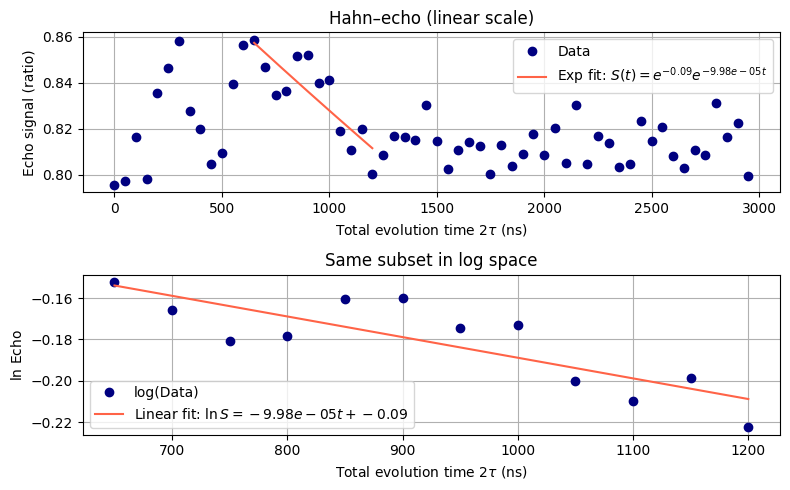
\includegraphics[width=0.7\textwidth]{../first_draft/figs/hahn.png} % Adjust path if needed
% \caption{Hahn echo decay.}
% \end{figure}
\end{frame}

%------------------------------------------------

% Optional: Add Conclusion Section
% \section{Conclusion}
% \begin{frame}
% \frametitle{Conclusion}
% \begin{itemize}
%     \item Summary of key results ($g^{(2)}(0)$, $\gamma_e$, $\Omega_R$, $T_2$)
%     \item Demonstrated optical characterization and coherent control.
%     \item Importance for quantum technologies.
% \end{itemize}
% \end{frame}

%------------------------------------------------
% Optional: Add references using BibTeX

\begin{frame}[allowframebreaks] % allowframebreaks makes bibliography span multiple frames if needed
\frametitle{References}
\bibliography{refs} % Adjusted path to your .bib file
\bibliographystyle{ieeetr} % Choose a suitable bibliography style
\end{frame}

%------------------------------------------------

\end{document} 